\chapter{Kademlia}
\textbf{Kademlia} is a protocol used by some of the largest public DHTs
\note{
   \ns
\begin{itemize}
   \item BitTorrent Mainline DHT
   \item Ethereum P2P network
   \item IPFS
\end{itemize}
}
{It has three key charateristics which are not offered by other DHTs\ns
\begin{enumerate}
   \item routing information spreads automatically as a side-effect of lookups
   \item flexibility to send multiple requests in parallel to speed up lookups by
   avoiding timeout delays (parallel routing)
   \item iterative routing
   \note{At each routing step of the query, the queried node sends a report to the starting querying node, even if it could not answer the query.}
\end{enumerate}}

\section{Structure}
\begin{paracol}{2}
   \colfill
   Kademlia exploits the leaves of a complete binary \textbf{Trie}\footnote{k-ary search tree and prefix tree} to define the logical identifier space;

   Note that not all leaves correspond to nodes (peers). In Fig. \ref{fig:kademlia_trie}, \ul{only the \textbf{circled} leaves are nodes}.
   \colfill
   \switchcolumn

   \begin{figure}[htbp]
      \centering
      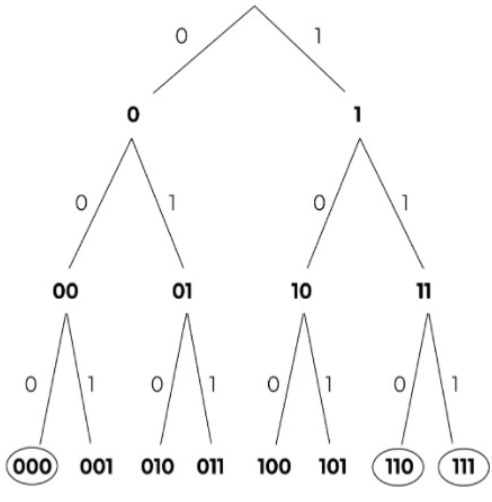
\includegraphics{images/kademlia_trie.png}
      \caption{Trie}
      \label{fig:kademlia_trie}
   \end{figure}
\end{paracol}

\newpage
\subsection{Assigning keys to leaves}
The rule to partition the keys (content) among the nodes must respect the rules of \textit{consistent hashing}.

\begin{paracol}{2}
   \colfill
   \begin{definition}[Partitioning rule]
      A key is assigned to the node with the
      \textit{``\ul{lowest} common ancestor''}:\\
      Find the longest prefix between the
      key and the node identifier, and then assign the key to such node.
   \end{definition}
   \colfill
   \switchcolumn
   \begin{figure}[htbp]
      \centering
      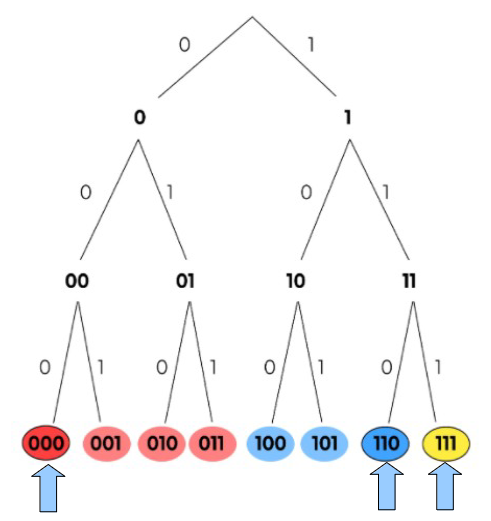
\includegraphics[width=0.45\columnwidth]{images/kademlia_leaves01.png}
      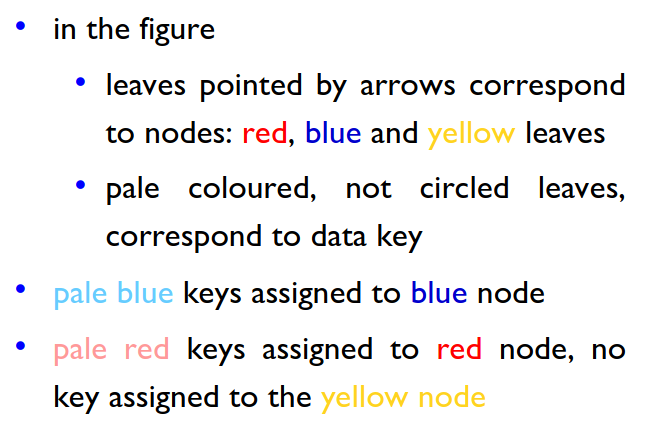
\includegraphics[width=0.45\columnwidth]{images/kademlia_leaves02.png}
      \label{fig:kademlia_leaves}
   \end{figure}
\end{paracol}

\section{Distance - XOR Metric}
In Fig. \ref{fig:kademlia_leaves} the assignment of keys to blue nodes instead of yellow ones is arbitrary, since the two nodes ``tie'' for the longest common prefix challenge, leading to no keys being assigned to the yellow nodes.\\
The problem may be solved by assigning keys to the node with the \textit{``closest''} identifier to the key.\\
\begin{center}
   \textit{\ul{How to compute the \textbf{distance} between two nodes?}}
\end{center}
To solve this problem, Kademlia uses the \textbf{XOR metric}.
The XOR metric consists in computing the XOR between a key and a node ID, and interpreting the result as an integer to get the distance.\\
This ensures that there is a unique closest node to a key, and that the distance between two nodes is the same in both directions.

\section{Routing Table}
In order to look for data, Kademlia's key idea is to \ul{store a logarithmic number of node IDs and their corresponding IP} addresses and some contact taken from the identifier trie.

\begin{figure}[htbp]
   \centering
   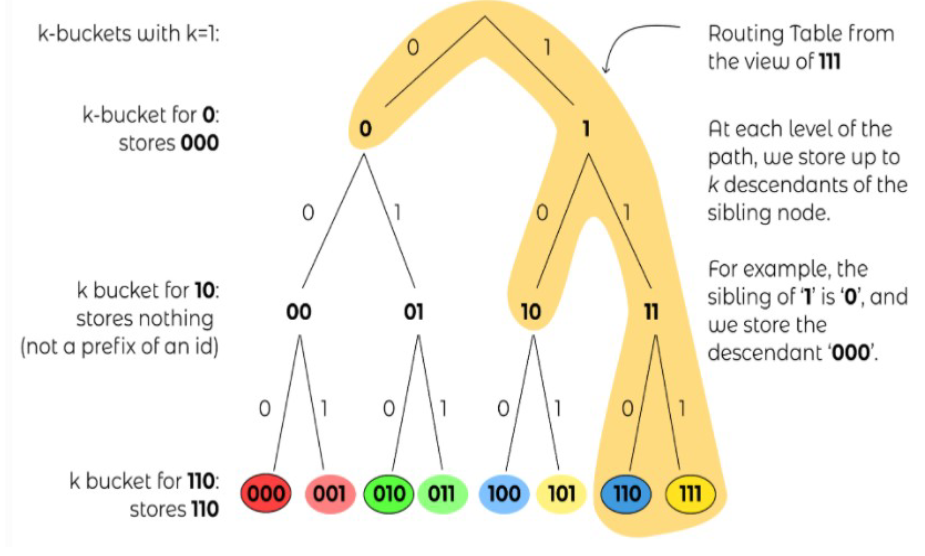
\includegraphics{images/kademlia_routingtable.png}
   \caption{Neighbours and buckets}
   \label{fig:kademlia_routingtable.png}
\end{figure}


Each k-bucket corresponds to a prefix and covers a subset of the identifier space: the set of all k-buckets covers the whole identifier space which $2^m$, with $m$\footnote{$m=160$ in Kademlia} the length of an identifier; more precisely the $i$-th bucket covers the range $[2^i, 2^{i+1})$, so as $i$ increases, so does the range of the bucket, exponenetially.\\
The first entries of the routing table correspond to peers sharing a long prefix
with the owner of the routing table; the last entries instead of the routing table correspond to peers sharing a smaller prefix, and cover a larger set of identifiers.
The value of $k$ is defined such that the probability that a crash of more of $k$ nodes is a rare event.
\ul{Nodes in each bucket are maintained ordered such that \textit{least recently contacted nodes are in the first positions of the list}}.
\newpage
\begin{figure}[htbp]
   \centering
   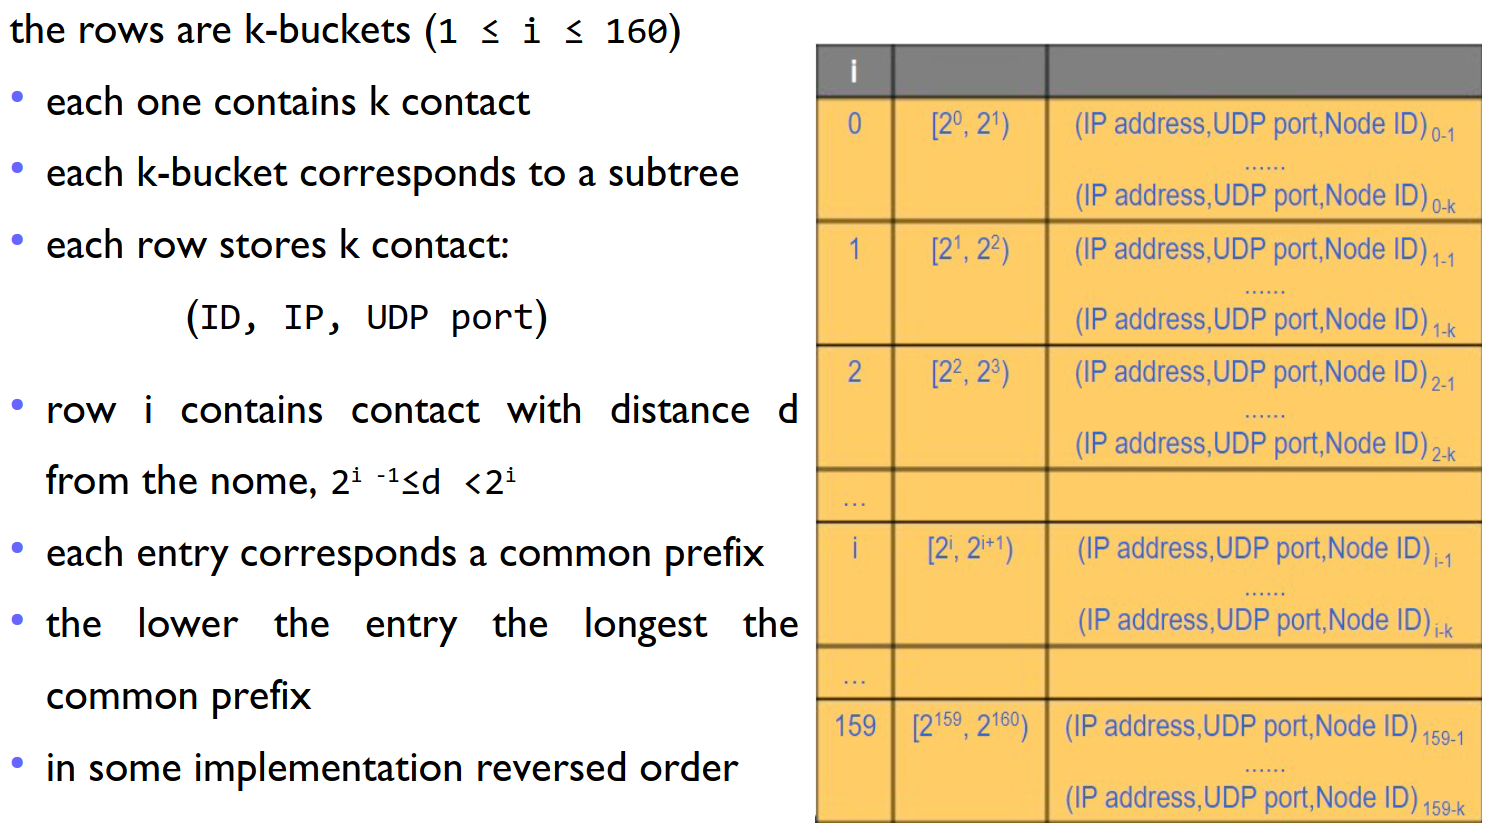
\includegraphics[width=0.45\columnwidth]{images/kademlia_routing_table1.png}
   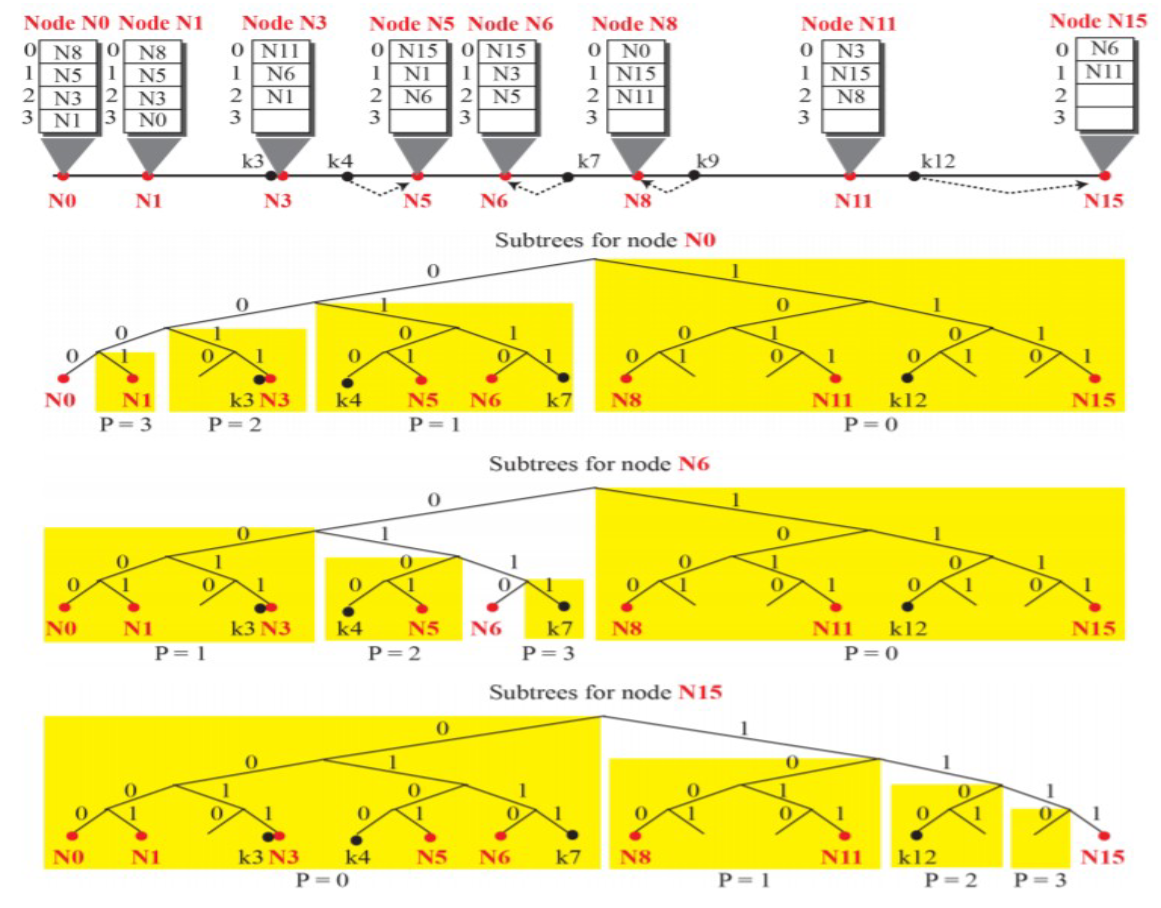
\includegraphics[width=0.45\columnwidth]{images/kademlia_routing_table2.png}
   \label{fig:kademlia_routing_table}
   \caption{Deeper into Routing Tables and buckets}
\end{figure}

\subsection{Routing Strategies}
In \textbf{iterative routing} the node $n$ sending the lookup request manages the whole search process.
At each routing step  $n$ receives a reply including a notification of the next routing step.

In \textbf{recursive routing} the node $n$ sending the lookup request delegates the search process to the node replying to the request.

\textbf{Parallel routing} is a strategy that allows the requester to send multiple requests in parallel to speed up the lookup process.
% //TODO

\section{Key Lookup}

{The idea for key lookup is:\ns
\begin{enumerate}
   \item Find the closest node to the key in your routing table, computing the XOR distance in case of ties
   \item While the closest node you know of does not have the key and has not already responded
   \begin{enumerate}
      \item Ask the closest node you know of, for the key or a closer node
      \item If the closest node responds with a closer node, update your closest nodes set. (i.e. current bucket)
   \end{enumerate}
\end{enumerate}}
At each iteration, the XOR metric is reduced by $\sfrac{1}{2}$ and results in smaller size k-buckets

\begin{figure}[htbp]
   \centering
   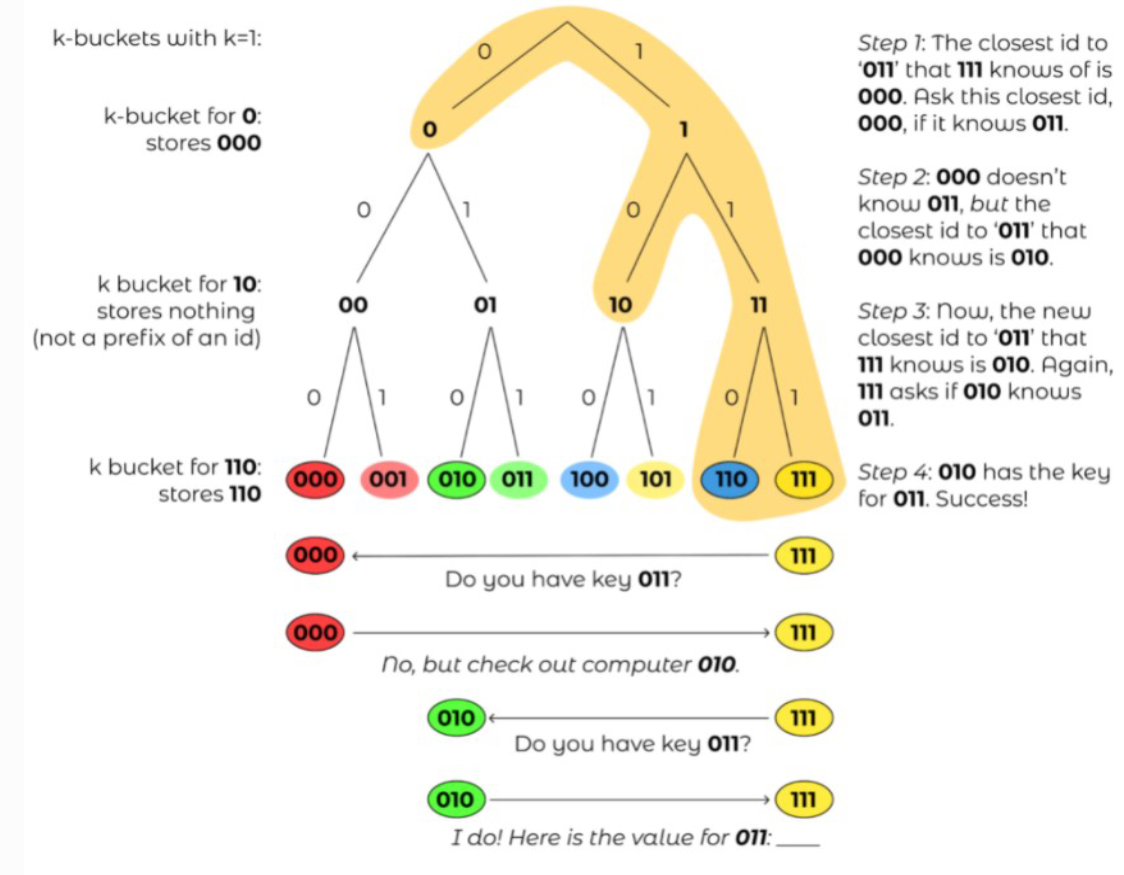
\includegraphics{images/kademlia_lookup.png}
   \caption{Kademlia Lookup at a glance}
   \label{fig:kademlia_lookup}
\end{figure}

\section{Protocol Messages}
\begin{enumerate}
   \item \texttt{FIND\_NODE $v\longrightarrow w$} (T) (v,w nodes, T target of the look up)\\
   the recipient of the message (w) returns k (IP address, UDP port, Node
   ID) triples for the k nodes it knows about closest to the target T.
   
   these triples can come from a single k-bucket, or they may come from multiple
   k-buckets if the closest k-bucket is not full.
   
   in any case, the recipient must return k items, unless there are fewer than k
   nodes in all its k-buckets combined, in which case it returns every node it
   knows about 



   
   \item \texttt{FIND\_VALUE} $v \longrightarrow w(T)(v,w \textit{ nodes}, T \textit{ value looked up})$\\
   in: T, 160-bit ID representing a value
   
   out:
   if a value corresponding to T is present in the queried node (w), the
   associated data is returned
   otherwise it is equivalent to \texttt{FIND\_NODE} and w returns a set of k triples
   
   If \texttt{FIND\_VALUE} returns a list of other peers, it is up to the requester to continue
   searching for the desired value from that list
   
   \item \texttt{PING} $v \longrightarrow w$
   
   probe node w to see if its online
   \item \texttt{STORE} $v \longrightarrow w$ $(Key, Value)$
   
   instructs node w to store a $\langle key, value \rangle$ pair
   
   the node has been retrieved through a
\end{enumerate}
The actual \textbf{Lookup algorithm} is based on \texttt{FIND\_NODE}.
many \texttt{FIND\_NODE} can be executed in parallel, according to $\alpha$ that is a system-wide concurrency parameter.
\note{With $\alpha = 1$, the lookup algorithm is similar to \textit{Chord}, one step progress each time}
\note{Lookup procedure is the same for \texttt{FIND\_VALUE} and \texttt{FIND\_NODE}}